The F$(v1)$ execution engine had chunks of memory leaks. The blocks of heap
memory were still reachable when the engine exited. As such, it was essential
to profile the engine to properly deallocate all blocks before exit. Listing
\ref{lst:fv2-engine-profile} shows the valgrind profile output of both
versions.  The $20kB$ of created and still living blocks in the current
snapshot are due two libraries. The \texttt{dyld} library makes $81$
\texttt{malloc} invocations that are not free'd by the library as shown in
figure \ref{fig:profile-invocations}. On GNU/Linux, \texttt{dyld} is replaced
is by \texttt{dlopen} which does not have this issue. The other set of
libraries, \texttt{libsystem\_c, libsystem\_notify, libdispatch} make $10$
\texttt{malloc} invocations that are again not free'd as shown in figure
\ref{fig:profile-invocations}.  These \texttt{malloc} calls invoke
\texttt{localtime(\ldots)} which uses \texttt{tzset(...)} to initialize and
return \texttt{struct tm*}. This structure is never free'd apparantely due to
a bug in these libraries.

\begin{figure}[ht!]
\centering
\subfigure{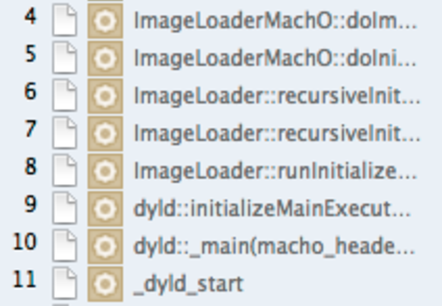
\includegraphics[width=.40\linewidth]{figures/dyld}}\quad
\subfigure{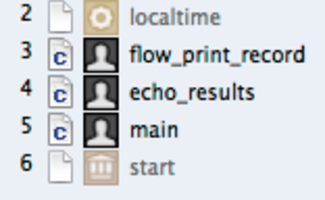
\includegraphics[width=.40\linewidth]{figures/localtime}}\\
\caption{F$(v2)$: Backtrace of Living on Exit Blocks}
\label{fig:profile-invocations}
\end{figure}

\lstset{caption=F$(v2)$: Valgrind-based Engine Profiling,
				tabsize=2, language=bash, numbers=left,stepnumber=1,
        basicstyle=\tiny\ttfamily, numberstyle=\ttfamily\color{gray},
        keywordstyle=\color{blue}, frame=shadowbox,
        rulesepcolor=\color{black}, label=lst:fv2-engine-profile,
        aboveskip=20pt, captionpos=b, upquote=true}
\begin{lstlisting}
$ git checkout v0.1; make
$ valgrind bin/engine queryfile tracefile

==19000== LEAK SUMMARY:
==19000==    definitely lost: 6,912 bytes in 472 blocks
==19000==    indirectly lost: 0 bytes in 0 blocks
==19000==      possibly lost: 0 bytes in 0 blocks
==19000==    still reachable: 124,607 bytes in 710 blocks
==19000==         suppressed: 0 bytes in 0 blocks

$ git checkout master; make
$ valgrind bin/engine queryfile tracefile

==19164== LEAK SUMMARY:
==19164==    definitely lost: 0 bytes in 0 blocks
==19164==    indirectly lost: 0 bytes in 0 blocks
==19164==      possibly lost: 0 bytes in 0 blocks
==19164==    still reachable: 20,228 bytes in 37 blocks
==19164==         suppressed: 0 bytes in 0 blocks
\end{lstlisting}

